\section{Métodos en diferencias finitas}
En esta sección vamos a ver métodos en diferencias finitas para distintos tipos de ecuaciones. Estos métodos se utilizan para calcular soluciones aproximadas a las ecuaciones diferenciales aproximando derivadas.

\subsection{Ecuaciones parabólicas en una dimensión espacial.}

Las ecuaciones parabólicas en una dimensión espacial son un tipo de ecuaciones cuya solución $u(x,t)$ es una función de dos variables: la variable espacial $x$ de una dimensión y una variable temporal $t$. Estas ecuaciones tienen la siguiente forma para $x\in I$ y $t>0$:
$$e(x,t)u_t = \underbrace{\frac{\partial}{\partial x} \left(a(x,t)\frac{\partial u}{\partial x}\right)}_{t_d} + \underbrace{b(x,t)\frac{\partial u}{\partial x}}_{t_c}+\underbrace{c(x,t)u}_{t_n} + \underbrace{d(x,t)}_{t_f}$$
donde $I$ es un intervalo dado. Los términos de la ecuación son los siguentes:
\begin{itemize}
	\vspace{-3mm}
	\item $a,b,c,d,e$: funciones proporcionadas.
	\item $t_d$: término de difusión.
	\item $t_c$: término conectivo.
	\item $t_n$: término de reacción.
	\item $t_f$: término fuente.
\end{itemize}

Vamos a tratar con los siguientes tipos de condiciones de contorno: la condición de Dirichlet y la condición de Neumann:
\begin{itemize}
	\item \textbf{Condición de Dirichlet:}	
	Una condición de tipo Dirichlet tiene la siguiente forma para dos funciones temporales $f_1, f_2$ y dos puntos $a,b$:
	\begin{equation*}
		\left\{
		\begin{array}{l l}
			u(a,t) = f_1(t)\\
			u(b,t) = f_2(t)\\
		\end{array}
		\right.
	\end{equation*}
	Se denominan condiciones homogéneas si $f_1=f_2=0$.
	\item \textbf{Condición de Neumann:}
	Una condición de tipo Neumann tiene la siguiente forma para dos funciones temporales $g_1, g_2$ y dos puntos $a,b$:	
	\begin{equation*}
		\left\{
		\begin{array}{l l}
			u_x(a,t) = g_1(t)\\
			u_x(b,t) = g_2(t)\\
		\end{array}
		\right.
	\end{equation*}
	Se denominan condiciones homogéneas si $g_1=g_2=0$.
\end{itemize}

\subsubsection{La ecuación del calor}
La ecuación del calor es un caso particular de ecuación parabólica en una dimensión espacial en la que $u(x,t)$ representa el valor de la temperatura en el punto $x$ en tiempo $t$. La ecuación es la siguiente:
$$u_t = u_{xx}$$

Supongamos que tenemos una barra unidimensional de cualquier material cuyos extremos se localizan en los puntos $0$ y $1$ y que tiene como temperatura inicial en cada punto la que indica una función proporcionada $u_0(x)$. En este caso, el intervalo $I$ se define como $I = (0,1)$.

El problema es el siguiente:
\begin{equation*}
	\left\{
	\begin{array}{l l l}
		u_t = u_{xx} & x\in I, t>0\\
		u(0,t) = u(1,t) = 0 & \text{Temperatura en los extremos.}\\
		u(x,0) = u_0(x) & \text{Temperatura en el tiempo inicial.}\\
	\end{array}
	\right.
\end{equation*}

Vamos a utilizar el método de separación de variables para encontrar la solución. Para ello, supongamos que la solución se puede representar como el producto de dos funciones $f(x)$ y $g(t)$, es decir $u(x,t) = f(x)g(t)$.

Como $u_t = u_{xx}$, derivando $u(x,t)$ respecto a $t$ una vez, respecto a $x$ dos veces e igualando términos, obtenemos:
$$f(x) \dot{g}(t) = \ddot{f}(x) g(t)$$
de donde si despejamos obtenemos una igualdad en la que el término izquierdo depende de $t$ y el derecho de $x$. Si se deriva el término izquierdo respecto a $x$ se obtiene cero igualmente que si derivamos el derecho respecto a $t$. Con esto obtenemos que los términos no dependen ni de $x$ ni de $t$, luego son iguales a una constante que por comodidad para cálculos posteriores denotaremos como $-K^2$:
$$\frac{\dot{g}(t)}{g(t)} = \frac{\ddot{f}(x)}{f(x)} = cte = -K^2$$
Tenemos entonces dos ecuaciones diferenciales ordinarias:
\begin{equation*}
	\left\{
	\begin{array}{l}
		\ddot{f}(x) = -K^2 f(x)\\
		\dot{g}(t) = -K^2 g(t)\\
	\end{array}
	\right.
\end{equation*}
Al resolver las ecuaciones se obtiene
\begin{equation*}
	\begin{array}{l}
		f(x) = Acos(Kx) + Bsin(Kx)\\
		g(t) = e^{-K^2 t}
	\end{array}
\end{equation*}
Las condiciones de contorno establecían que $u(0,t) = u(1,t) = 0$. 
Dado que hemos supuesto que $u(x,t) = f(x)g(t)$ se esta imponiendo que $f(0) = f(1) = 0$, lo que implica que
\begin{equation*}
	\left\{
	\begin{array}{l}
		f(0) = Acos(0) + Bsin(0) = 0\\
		f(1) = Acos(K) + Bsin(K) = 0\\
	\end{array}
	\right.
\end{equation*}
Esto sólo puede ocurrir si
\begin{equation*}
	\left\{
	\begin{array}{l l}
		A = 0 & \\
		K = m\pi & m\in\mathbb{Z}\\
	\end{array}
	\right.
\end{equation*}
Como la condición se satisface $\forall m \in \mathbb{Z}$ tenemos infinitas funciones $f_m, g_m$ que cumplen la condición. Luego para cada $m$, se tiene que $u_m(x,t) = f_m(x)g_m(t)$ es solución del problema de contorno.
Por tanto también lo es
$$u(x,t) = \sum_{m=1}^\infty B_m e^{-(m\pi)^2 t} sin(m\pi x)$$
donde $B_m$ es una constante que depende de $m$.

Sin embargo, hasta ahora sólo se han tenido en cuenta las condiciones de contorno y no la condición inicial. Hay que imponer dicha condición para obtener una solución al problema. Dicha condición establece que $u(x,0) = u_0(x)$ siendo $u_0$ una función proporcionada.
Tenemos que:
$$u(x,0) = u_0(x) = \sum_{m=1}^\infty B_m sin(m\pi x)$$
Esto nos dice que los términos $B_m$ son los coeficientes del desarrollo en senos de la serie de Fourier de $u_0$.
Es decir, que:
$$\int_0^1 u_0(x) sin(m\pi x) = \frac{B_m}{2}$$ para cada $m\in\mathbb{Z}$. Obteniendo así $$B_m = 2\int_0^1 u_0(x) sin(m\pi x)$$
Finalmente, la solución general al problema completo es:
$$u(x,t) = \sum_{m=1}^\infty B_m e^{-(m\pi)^2 t} sin(m\pi x)$$ donde $B_m$ tiene la expresión definida anteriormente.

En caso de que tuviesemos un dato inicial $u_0$ y quisiésemos hallar la solución del problema de la ecuación del calor tendríamos que

\begin{itemize}
	\item Hallar el valor aproximado de la serie, para lo cual se evalua cada término para cada $m$ y se trunca la serie cuando se considere que los términos restantes aportan un error insignificante al resultado.
	\item Para lo anterior es necesario hallar el valor de $B_m$ para cada iteración, bien de forma exacta si es posible o mediante métodos numéricos. Una opción sería utilizar cuadratura numérica:
	$$\int_a^b f(x) \approx \sum_{j=0}^k w_j f(x_j)$$
\end{itemize}

\paragraph{Método explícito}\mbox{}

En este apartado se va a describir una forma explícita del método en diferencias finitas para la ecuación del calor. En primer lugar se construyen dos particiones para cada variable, una para el intervalo $(0,1)$ y otra para el intervalo $(0,t_f)$ donde $t_f$ representa el tiempo final, de forma que $x\in(0,1)$ y $t\in(0,t_f)$.

Cada partición se define a través de los valores del paso, que son
\begin{equation*}
	\begin{array}{lll}
		\Delta x = \frac{1}{J}& \textbf{y} & \Delta t = \frac{t_f}{N}
	\end{array}
\end{equation*}
donde $J,N\in\mathbb{N}$, es decir, que se obtienen $N+1$ puntos en $(0,1)$ y $J+1$ puntos en $(0,t_f)$:
\begin{align*}
0=x_0<x_1<\hdots<x_J = 1\\
0=t_0<t_1<\hdots<t_N = t_f
\end{align*}

En la figura \ref{fig:calor_1} se puede ver el particionado del espacio para las variables de $u(x,t)$. En color rojo se muestran posicionados los datos de contorno, que en este caso son todos $0$ puesto que tenemos $u(0,t) = u(1,t) = 0$ como condición inicial. En color azul se muestran posicionados los datos iniciales, que corresponden para cada punto a los valores de la función proporcionada $u_0(x)$. 

\begin{figure}[h]
	\centering
	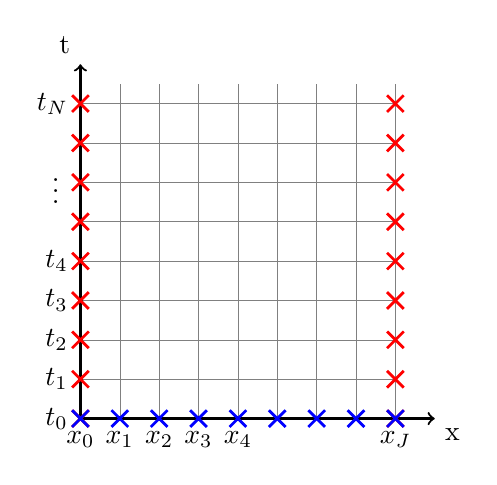
\begin{tikzpicture}[domain=0:4]
	%Grid
	\draw[step=5mm,very thin,color=gray] (0,0) grid (4,4.25);
	%Axis
	\draw[thick,->] (0,0) -- (4.5,0) node[below right] {x};
	\draw[thick,->] (0,0) -- (0,4.5) node[above left] {t};
	\foreach \x in {0,1,2,3,4}
	\draw (5*\x mm,1pt) -- (5*\x mm,-1pt) node[below] {$x_\x$};
	\node[below] at (3,-4pt){$\hdots$};
	\node[below] at (4,-1pt){$x_J$};
	\foreach \y in {0,1,2,3,4}
	\draw (1pt,5*\y mm) -- (-1pt,5*\y mm) node[left] {$t_\y$};
	\node[left] at (-4pt,3){$\vdots$};
	\node[left] at (-1pt,4){$t_N$};
	%Data
	\foreach \x in {0,...,8}{
		\draw[rotate around={45:(0,5*\x mm)},red, line width=1pt] (0.15,5*\x mm) -- (-0.15,5*\x mm);
		\draw[rotate around={135:(0,5*\x mm)},red, line width=1pt] (0.15,5*\x mm) -- (-0.15,5*\x mm);
	}
	\foreach \x in {0,...,8}{
		\draw[rotate around={45:(4,5*\x mm)},red, line width=1pt] (4.15,5*\x mm) -- (3.85,5*\x mm);
		\draw[rotate around={135:(4,5*\x mm)},red, line width=1pt] (4.15,5*\x mm) -- (3.85,5*\x mm);
	}
	\foreach \y in {0,...,8}{
		\draw[rotate around={45:(5*\y mm,0)},blue, line width=1pt] (5*\y mm,0.15) -- (5*\y mm,-0.15);
		\draw[rotate around={135:(5*\y mm,0)},blue, line width=1pt] (5*\y mm,0.15) -- (5*\y mm,-0.15);
	}
	\end{tikzpicture}
	\caption{Datos iniciales y de contorno}
	\label{fig:calor_1}
\end{figure}

Antes de estudiar el método, vamos a definir qué notación se va a utilizar durante toda la descripción del mismo. 
\begin{mdframed}
	\textbf{Notación:}
	\begin{itemize}
		\vspace{-3mm}
	\item $U_j^n$ representa el valor \textbf{obtenido por el método} de la función $u$ evaluada en $x_j,t_n$.
	\item $u_j^n$ representa el valor \textbf{real} de la función $u$ evaluada en $x_j,t_n$.
	\end{itemize}
	Esta notación va a utilizarse de aquí en adelante en todo lo que sigue.
\end{mdframed}

Empezemos recordando que las condiciones de contorno eran las siguientes:
$$u(0,t) = u(1,t) = 0$$
lo que implica que nuestro método ha de cumplir
\begin{equation*}
	\left\{
	\begin{array}{l}
	U_0^n = u_0^n = 0, n\ge 0\\
	U_J^n = u_J^n = 0, n\ge 0
	\end{array}
	\right.
\end{equation*}

Supongamos que $u(x)$ es una solución del problema de la ecuación del calor con los datos iniciales y las condiciones de contorno porporcionados. Podemos aproximar las derivadas $u_{xx}$ y $u_t$ de la siguiente forma:
\begin{align*}
		u_{xx}(x_j, t_n) &\approx \frac{u(x_{j+1}) - 2u(x_j, t_n) + u(x_{j-1}, t_n)}{(\Delta x)^2}\\
		u_t(x_j, t_n) &\approx \frac{u(x_j, t_{n+1})-u(x_j,t_n)}{\Delta t}
\end{align*}

Tenemos un valor aproximado para $u_{xx}$ y $u_t$, luego sabiendo que la ecuación del calor es $u_t = u_{xx}$, podemos construir el siguiente método:
\begin{equation*}
	\frac{U_j^{n+1}-U_j^n}{\Delta t} =  \frac{U_{j+1}^n-2U_j^n+U_{j-1}^n}{(\Delta x)^2}
\end{equation*}
para $n\ge  0$ y $j=1,\hdots ,J-1$.

A partir de aquí, se puede observar que en el método anterior se puede despejar el término que da el valor aproximado de la función en el punto $j$ y en tiempo $n+1$, obteniendo el método explícito:

\begin{mdframed}
	\textbf{Método explícito}
	$$U_j^{n+1} = U_j^n+\nu\left(U_{j+1}^n - 2 U_j^n + U_{j-1}^n\right)$$
	donde $\nu = \frac{\Delta t}{(\Delta x )^2}$
\end{mdframed}

En lo que sigue, utilizando el desarrollo de la serie Taylor, se va a estudiar qué orden tiene esta aproximación.

\subparagraph{Orden del método explícito} 
\mbox{}

Vamos a hallar el desarrollo de Taylor alrededor del punto $x_j, t_n$ del término temporal del método. Vemos que:
$$u(x_j, t_{n+1}) = u(x_j, t_n) + u_t(x_j, t_n)\Delta t +\frac{u_{tt} (x_j,t_n)}{2}\Delta t ^2 + O\left((\Delta t)^3\right)$$

luego:
$$\frac{u(x_j,t_{n+1}) - u(x_j, t_n)}{\Delta t} = u_t(x_j,t_n) + \underbrace{\frac{\Delta t}{2} u_{tt}(x_j,t_n) + O\left((\Delta t)^2\right)}_{\text{error}}$$

Ahora vamos a repetir lo anterior, pero esta vez desarrollaremos la serie de Taylor alrededor del punto $x_j, t_n$ del término espacial del método. 

Tenemos que:
\begin{align*}
u(x_{j+1}, t_n) &= u(x_j,t_n) + u_x(x_j,t_n)\Delta x + u_{xx}(x_j,t_n)\frac{\Delta x^2}{2}\\ &+\  u_{xxx}(x_j,t_n)\frac{\Delta x^3}{3!}  + \hdots\\
\end{align*}

y por otro lado
\begin{align*}
u(x_{j-1},t_n) &= u(x_j, t_n) - u_x(x_j,t_n)\Delta x + u_{xx}(x_j,t_n)\frac{(\Delta x)^2}{2}\\ &-\ u_{xxx}(x_j, t_n)\frac{(\Delta x)^3}{3!} + u_{xxxx}(x_j,t_n)\frac{(\Delta x)^4}{4!} + \hdots
\end{align*}

finalmente obtenemos:
$$\frac{u(x_{j+1}, t_n) - 2u(x_j,t_n) + u(x_{j-1},t_n)}{(\Delta x)^2} = u_{xx}(x_j,t_n) + \underbrace{ u_{xxxx}(x_j, t_n)\frac{\Delta x^2}{12} + O\left((\Delta x)^4\right)}_{\text{error}}$$

Como conclusión tenemos que el método explícito utiliza una diferencia finita de primer orden para aproximar la derivada temporal y una diferencia finita de segundo orden para aproximar la derivada espacial.

\subparagraph{Error de truncación}\mbox{}

\begin{defn}[Error de truncacion]
Se llama error de truncación del método numérico al residuo que se obtiene cuando se aplica el método a la solución exacta.
\end{defn}

El error de truncación del método explícito, atendiendo a la definición anterior, tiene la expresión:
$$T(x_j,t_n) = \frac{u(x_j,t_{n+1})-u(x_j,t_n)}{\Delta t} - \frac{u(x_{j+1},t_n)-2u(x_j,t_n)+u(x_{j-1},t_n)}{\Delta x^2}$$

Supongamos que $u(x,t)$ es la solución exacta del problema de la ecuación del calor. Vamos a hallar, mediante el desarrollo de Taylor, el error de truncación del método explícito:
\begin{align*}
T(x_j,t_n) &= \frac{u(x_j,t_{n+1})-u(x_j,t_n)}{\Delta t} - \frac{u(x_{j+1},t_n)-2u(x_j,t_n)+u(x_{j-1},t_n)}{\Delta x^2}\\ 
& =  u_t(x_j,t_n) + u_{tt}(x_j,t_n)\frac{\Delta t}{2} + O \left((\Delta t)^2\right) \\
& - u_{xx}(x_j,t_n) + u_{xxxx}(x_j,t_n)\frac{\Delta x^2}{12} + O\left((\Delta x)^4\right)\\ 
& =  u_{tt}(x_j,t_n)\frac{\Delta t}{2} -  u_{xxxx}(x_j,t_n)\frac{\Delta x^2}{12} + O\left((\Delta t)^2\right) + O\left((\Delta x)^4\right)
\end{align*}

En el último paso, se ha tenido en cuenta que $u_t = u_{xx}$. Otra forma escribir el error de truncación es la que sigue:
$$T_j^n = \Delta t \left(\frac{u_{tt}(x_j,t_n)}{2}- \frac{1}{12\nu} u_{xxxx}(x_j,t_n)\right) + O\left((\Delta t)^2\right) + O\left((\Delta x)^4\right)$$

Si tomamos $\xi_n \in (t_n,t_{n+1})$ y $\eta_j \in (x_{j-1}, x_{j+1})$ podemos eliminar los términos para la comparación asintótica:
$$T_j^n = \Delta t \left(\frac{u_{tt}(x_j,\xi_n)}{2}- \frac{1}{12\nu} u_{xxxx}(\eta_j,t_n)\right)$$

\subparagraph{Cota para el error de truncación}\mbox{}

Si tomamos $M_{tt}$ y $M_{xxxx}$ como cota para $u_{tt}$ y $u_{xxxx}$, tenemos el error de truncación acotado como sigue:

$$|T_j^n| \le \Delta t \left(\frac{M_{tt}}{2} + \frac{M_{xxxx}}{12{\nu}}\right)$$

Dado que la ecuación del calor establece que $u_{t} = u_{xx}$, entonces, asumiendo regularidad en la solución, se tiene que $(u_t)_{t} = (u_{t})_{xx} = u_{xxxx}$. 

Como caso particular, si tomamos $\nu = 1/6$ se cumple :
$$T_j^n = \Delta t\cdot 0 + O\left((\Delta t)^2\right) + O\left((\Delta x)^4\right) = O\left((\Delta t)^2\right)$$
obteniendo así orden 2 para el error de truncación.

\subparagraph{Convergencia del método}\mbox{}

El método explícito es consistente porque el error de truncación tiende a cero cuando $\Delta t \to 0$.
Además es incondicionalmente consistente, lo que quiere decir que $T_j^n$ tiende hacia cero independientemente de los valores de $\Delta t$ y $\Delta x$ (más concretamente de su relación $\nu = \frac{\Delta t}{(\Delta x)^2}$).

En esta sección se va a estudiar la convergencia del método, antes de ello, vamos a ver qué necesitamos para demostrar que es convergente.

\begin{prop}
	$$\text{Estabilidad} + \text{Consistencia} \iff \text{Convergencia}$$
\end{prop} 

A partir de esta proposición y dado que el método es incondicionalmente consistente, basta que sea estable para que sea convergente.

\begin{prop}
$$\text{El método es estable} \iff \nu \le \frac{1}{2}$$
\end{prop}

\begin{proof}
	
Vamos a ver, utilizando el principio del máximo, que si $\nu < \frac{1}{2}$, el método es estable. Tenemos que:
\begin{align*}
u_j^{n+1} &= u_j^n + \nu (u_{j+1}^n-2u_j^n+u_{j-1}^n) + T_j^n \Delta t\\
U_j^{n+1} &= U_j^n + \nu (U_{j+1}^n-2U_j^n+U_{j-1}^n)
\end{align*}

Denotamos con $e_j^n$ al residuo del método, de forma que:
$$e_j^n = U_j^n - u_j^n$$

Calculamos el error de paso:
$$e_j^{n+1} = e_j^n + \nu (e_{j+1}^n-2e_j^n+e_{j-1}^n) - T_j^n \Delta t$$

Operando y suponiendo que $\nu \le \frac{1}{2}$ queda:
$$e_j^{n+1} = \nu e_{j+1}^n + \underbrace{(1-2\nu)}_{\ge 0} e_j^n + \nu e_{j-1}^n - T_j^n \Delta t$$

Ahora definimos
$$E^n = \max_{0\le j \le J} |e_j^n|$$

y acotamos el error:
\begin{equation*}
	\begin{array}{lll}
	|e_j^{n+1}| &\le& \nu|e_{j+1}^n| + (1-2\nu) |e_j^n| + \nu |e_{j-1}^n| +  \bar{T}\Delta t\\
	&\le& \nu E^n +(1-2\nu)E^n + \nu E^n + \bar{T}\Delta t\\
	&=& E^n + \bar{T} \Delta t
	\end{array}
\end{equation*}

Donde $$\bar{T} = \Delta t \left( \frac{M_{tt}}{2} + \frac{M_{xxxx}}{12\nu}  \right)$$

es decir, $\bar{T}$ es la cota para el error de truncación. 

\subparagraph*{Conclusión}\mbox{}

Como $E^0 = 0$ y $E^n = (n\bar{T})\Delta t \le t_f \bar{T}$, tenemos que $$E^n \to 0 \text{ cuando }\Delta t \to 0$$ 

es decir, el método es estable.
\end{proof}

Dado que hemos obtenido que el método es estable si $\nu <\frac{1}{2}$ e incondicionalmente consistente, tenemos que bajo la misma condición, el método es convergente.

\newpage

\subparagraph{Programación del método}\mbox{}

Sabemos que inicialmente tenemos los siguientes datos
\begin{equation*}
	\left\{
	\begin{array}{l r}
		u(0,t) = 0\\
		u(1,t) = 0\\
		u(x,0) = u_0(x)
	\end{array}
	\right.
\end{equation*}

Es decir, que disponemos de los datos iniciales (en tiempo $t=0$) y de contorno (cuando $x=0$ y $x=1$). Partiendo de ellos podemos calcular el resto de datos como ya hemos visto:

$$U_j^{n+1} = U_j^n+\nu\left(U_{j+1}^n - 2 U_j^n + U_{j-1}^n\right)$$

El algoritmo vectorial tendría la siguiente forma:
\begin{equation*}
	\begin{array}{l l l}
		\begin{bmatrix}
			U_1^{n+1}\\
			U_2^{n+1}\\
			\vdots\\
			U_{j-1}^{n+1}\\
		\end{bmatrix}
		=
		\begin{bmatrix}
			1-2\nu & \nu       &        & \\
			\nu    & \ddots    & \ddots & \\
			          & \ddots & \ddots & \nu\\
			          &        & \nu    & 1-2\nu\\
		\end{bmatrix}
		\begin{bmatrix}
			U_1^{n}\\
			U_2^{n}\\
			\vdots\\
			U_{j-1}^{n}\\
		\end{bmatrix}
	\end{array}
\end{equation*}

Gráficamente, lo que estamos realizando es obtener una aproximación (utilizando la aproximación de las derivadas) del siguiente punto de la partición en la derivada temporal a partir tres puntos en la derivada espacial (ver figura \ref{fig:calor_2}). De esta forma, sólo usando los datos iniciales y de contorno obtenemos un valor para cada uno de los puntos del mallado.

\begin{figure}[h]
	\centering
	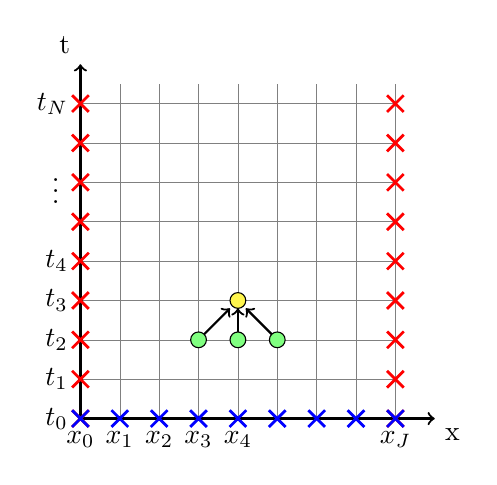
\begin{tikzpicture}[domain=0:4]
	%Grid
	\draw[step=5mm,very thin,color=gray] (0,0) grid (4,4.25);
	%Axis
	\draw[thick,->] (0,0) -- (4.5,0) node[below right] {x};
	\draw[thick,->] (0,0) -- (0,4.5) node[above left] {t};
	\foreach \x in {0,1,2,3,4}
	\draw (5*\x mm,1pt) -- (5*\x mm,-1pt) node[below] {$x_\x$};
	\node[below] at (3,-4pt){$\hdots$};
	\node[below] at (4,-1pt){$x_J$};
	\foreach \y in {0,1,2,3,4}
	\draw (1pt,5*\y mm) -- (-1pt,5*\y mm) node[left] {$t_\y$};
	\node[left] at (-4pt,3){$\vdots$};
	\node[left] at (-1pt,4){$t_N$};
	%Data
	\foreach \x in {0,...,8}{
		\draw[rotate around={45:(0,5*\x mm)},red, line width=1pt] (0.15,5*\x mm) -- (-0.15,5*\x mm);
		\draw[rotate around={135:(0,5*\x mm)},red, line width=1pt] (0.15,5*\x mm) -- (-0.15,5*\x mm);
	}
	\foreach \x in {0,...,8}{
		\draw[rotate around={45:(4,5*\x mm)},red, line width=1pt] (4.15,5*\x mm) -- (3.85,5*\x mm);
		\draw[rotate around={135:(4,5*\x mm)},red, line width=1pt] (4.15,5*\x mm) -- (3.85,5*\x mm);
	}
	\foreach \y in {0,...,8}{
		\draw[rotate around={45:(5*\y mm,0)},blue, line width=1pt] (5*\y mm,0.15) -- (5*\y mm,-0.15);
		\draw[rotate around={135:(5*\y mm,0)},blue, line width=1pt] (5*\y mm,0.15) -- (5*\y mm,-0.15);
	}
		\draw[thick,->] (1.5,1) -- (1.9,1.4);
		\draw[thick,->] (2,1) -- (2,1.4);
		\draw[thick,->] (2.5,1) -- (2.1,1.4);
	\draw[fill=green!50!white, draw=black] (1.5,1) circle (1mm);
	\draw[fill=green!50!white, draw=black] (2,1) circle (1mm);
	\draw[fill=green!50!white, draw=black] (2.5,1) circle (1mm);
	\draw[fill=yellow!70!white, draw=black] (2,1.5) circle (1mm);
	\end{tikzpicture}
	\caption{Método en diferencias finitas: $U_j^{n+1} = U_j^n+\nu\left(U_{j+1}^n - 2 U_j^n + U_{j-1}^n\right)$}
	\label{fig:calor_2}
\end{figure}

\newpage
\subparagraph{Análisis de Fourier del método explícito}\mbox{}

Hemos visto que la solución general para el problema de la ecuación del calor tiene la siguiente forma:
$$u(x, t) = \sum_{m=1}^\infty B_m e^{-(m\pi)^2 t} sin(m\pi x)$$

Equivalentemente, podemos reescribir lo anterior del siguiente modo:
$$u(x,t) = \sum_{m=-\infty}^\infty B_m e^{-(m\pi)^2 t}e^{i(m\pi)x}$$

Para la solución teórica, los modos de Fourier $e^{-k^2t}$ y $e^{ikx}$ definiendo \framebox{$k=m\pi$} y \framebox{$m=-\infty,\hdots, \infty$}, son soluciones particulares.

Para realizar el análisis de Fourier del método explícito vamos a definir un factor $\lambda(k)$ al que llamaremos factor de amplifiación:
$$\lambda(k) \simeq e^{-k^2\Delta t}$$ 

Ahora buscamos $U_j^n$ de la forma
\begin{equation*}
	\begin{array}{l l l}
		U_j^n =\lambda^n e^{ik(j\Delta x)}&\simeq& \left[e^{-k^2\Delta t}\right]^n\ e^{ik(j\Delta x)}\\
				&=& e^{-k^2n\Delta t}\ e^{ik(j\Delta x)}\\
				&=& e^{-k^2t_n}\ e^{ikx_j}\\
	\end{array}
\end{equation*}

Sustituyendo en el método explícito tenemos que
$$\lambda^{n+1}e^{ik(j\Delta x)} =
\lambda^ne^{ik(j\Delta x)} + \nu\left[\lambda^n e^{ik(j+1)\Delta x}-2\lambda^n e^{ik(j\Delta x)}+\lambda^n e^{ik(j-1)\Delta x}\right]$$

Dividiendo por $\lambda^n e^{ik(j\Delta x)}$
\begin{equation*}
	\begin{array}{l l l}
		\lambda(k) & = & 1+\nu\left[e^{ik\Delta x} -2 + e^{-ik\Delta x}\right]\\
		& = & 1 + \nu \left[2cos(k\Delta x)-2\right]\\
		& = & 1 + \nu \left[2\left(1-2sin^2(\frac{k}{2}\Delta x)\right)-2\right]\\
		& = & 1 + \nu \left[-4sin^2(\frac{k}{2}\Delta x)\right]\\
	\end{array}
\end{equation*}

Tomando $U_j^n = \lambda(k)^n e^{ikj\Delta x}$ se verifica el método y como aproximación tomamos
$$U_j^n = \sum_{m=-\infty}^\infty B_m \lambda(k)^n e^{ikj\Delta x}$$

\subparagraph*{Comportamiento cualitativo de $\lambda(k)$.}\mbox{}

El método presenta insestabilidad si $|\lambda(k)| > 1$ dado que $$|\lambda(k)| > 1 \implies |\lambda(k)|^n \to \infty$$ 

Tenemos estabilidad si y sólo si $|\lambda(k)| \le 1$. Esto es equivalente a decir que podemos acotar dos aproximaciones numéricas del método en términos de los datos iniciales. Supongamos dos datos iniciales para $t=0$:
\begin{equation*}
	\left\{
	\begin{array}{l}
		u_0^{(1)}(x) = \sum_{m=1}^\infty B_m^1 e^{ikx}\\
		u_0^{(2)}(x) = \sum_{m=1}^\infty B_m^2 e^{ikx}
	\end{array}
	\right.
\end{equation*}

Obtenemos las aproximaciones de la solución los problemas partiendo de dichos datos:
\begin{equation*}
\left\{
\begin{array}{l}
	(U_j^n)^{(1)} = \sum_{m=-\infty}^\infty B_m^1 \lambda(k)^n e^{ik(j\Delta x)}\\
	(U_j^n)^{(2)} = \sum_{m=-\infty}^\infty B_m^2 \lambda(k)^n e^{ik(j\Delta x)}\\
\end{array}
\right.
\end{equation*}

La diferencia entre las dos aproximaciones es
$$(U_j^n)^{(1)} - (U_j^n)^{(2)} = \sum_{m=-\infty}^\infty (B_m^1-B_m^2) \lambda(k)^n e^{ik(j\Delta x)}$$

Tomando normas
$$\left|(U_j^n)^{(1)}-(U_j^n)^{(2)}\right| \le \left|\sum_{m=-\infty}^\infty (B_m^1-B_m^2) e^{ik(j\Delta x)}\right| = \left|u_0^{(1)}(x_j)-u_0^{(2)}(x_j)\right|$$

\subparagraph*{Comportamiento cuantitativo de $\lambda(k)$.}\mbox{}

Vamos a comparar $e^{-k^2\Delta t}$ y $\lambda(k)$. Para ello, desarrollamos las series de Taylor de ambos términos:

\begin{align*}
		e^{-k^2\Delta t} & =  1-k^2\Delta t + \frac{1}{2}k^4\Delta t ^2 + O(\Delta t ^3)\\
		\lambda(k) & =  1-4\nu sin^2(\frac{k}{2}\Delta x)\\
		& =  1-4\nu\left[\frac{k^2}{4}\Delta x^2 - \frac{1}{3}\frac{k^4}{16}\Delta x^4 + \hdots \right]\\
		& =  1-k^2\Delta t + \frac{k^4}{12}\Delta t \Delta x^2 + \hdots
\end{align*}

Obteniendo la diferencia
$$\lambda(k) - e^{-k^2\Delta t} = \frac{k^4\Delta t \Delta x^2}{12} - \frac{k^4\Delta t^2}{2} + O(\Delta t ^3)$$

En general
$\lambda(k) - e^{-k^2\Delta t} = O(\Delta t^2)$, es decir, que el método tiene orden 1 de consistencia.

Se puede ver mejor si lo reescribimos de la forma:
$$\lambda(k) - e^{-k^2\Delta t} = \left[\frac{k^4}{12\nu}-\frac{k^4}{2}\right]\Delta t^2 + O(\Delta t^3)$$

Vemos de nuevo que si $\nu = \frac{1}{6}$ se tiene orden 2 de consistencia.

\subparagraph*{Convergencia del método explícito} \mbox{}

Ya sabemos que 
$$\lambda(k) = 1-4\nu sin^2(\frac{k}{2}\Delta x)$$ 

y que tenemos estabilidad si y sólo si \framebox{$|\lambda(k)|\le 1$}. 

Analizando $\lambda(k)$ vemos que
$$|\lambda(k)| = \left|1-4\nu sin^2\left(\frac{k}{2}\Delta x\right)\right|\le \left|1-4\nu\right|$$

Vamos a distinguir dos casos
\begin{itemize}
	\item Si $1-4\nu\ge 0 \implies 1-4\nu \le 1$
	\item Si $1-4\nu < 0\implies |1-4\nu| = -1+4\nu < 1 \iff 4\nu \le 2 \iff \nu \le \frac{1}{2}$ 
\end{itemize}

En el caso inestable ($\nu > \frac{1}{2}$) la frecuencia más inestable es $k = J\pi$, donde se obtienen oscilaciones:
$$\lambda^n e^{ikj\Delta x} = \lambda^n e^{iJ\pi j\frac{1}{J}} = \lambda^n e^{i\pi j} = \lambda^n cos(\pi j)$$

Veamos otra forma para ver que el método converge utilizando análisis de Fourier.

Por un lado tenemos la solución del problema
\begin{equation*}
		u(x,t)  =  \sum_{m=-\infty}^{\infty} B_m e^{(-m\pi)^2t}e^{im\pi x}
\end{equation*}

Y por otro el dato inicial
\begin{equation*}
	u(x,t)  =  \sum_{m=-\infty}^{\infty} B_m e^{im\pi x}
\end{equation*}

En el método explícito teníamos
\begin{equation*}
	U_j^n  =  \sum_{m=-\infty}^{\infty} \lambda^n(k)B_m e^{ik j\Delta x}
\end{equation*}

Hallamos $e_j^n$:
\begin{equation*}
	e_j^n = U_j^n - u_j^n =  \sum_{m=-\infty}^{\infty} B_m e^{ik j\Delta x}\left(\lambda^n(k) - e^{-k^2n\Delta t}\right)
\end{equation*}

Vamos a probar que $\forall \varepsilon > 0$ $\exists \Delta t_0$ tal que si $\Delta t \le \Delta t_0 \implies |e_j^n| < \varepsilon$ con la condición impuesta de que $\nu\le\frac{1}{2}$.

Como hipótesis de regularidad asumimos que la serie de Fourier de $u(x)$ es absolutamente convergente en $[0,1]$.

Fijamos $\nu$ y $\varepsilon > 0$. Existe un $m_0$ tal que $$\sum_{|m|>m_0} |B_m|\le \frac{1}{4}\varepsilon$$

Vamos a analizar $|e_j^n|$ en dos partes:
\begin{equation*}
	|e_j^n| \le \underbrace{\sum_{|m|>m_0}|B_m|\left(|\lambda^n(k)|+\left|e^{-k^2n\Delta t}\right|\right)}_1 + \underbrace{\sum_{|m|\le m_0}|B_m|\left|\lambda^n(k)-e^{-k^2n\Delta t}\right|}_2
\end{equation*}

Antes de comenzar el análisis es necesario enunciar el siguiente lema.
\begin{lemma}
	$$|\lambda| \le 1\text{ y }|\nu|\le 1 \implies |\lambda^n-\nu^n|\le n|\lambda-\nu|$$
\end{lemma}

La demostración de este lema se realiza por inducción. Ahora estudiamos los dos términos de la expresión para $|e_j^n|$:

\begin{enumerate}
	\item Utilizando que $|\lambda(k)| \le 1$ se acota $(1)$ por $$\sum_{|m|>m_0}2|B_m|$$
	\item Usando el lema llegamos a que
	$$\sum_{|m|\le m_0}{|B_m|\cdot n\cdot \left|\lambda(k)-e^{-k^2\Delta t}\right|} \le \sum_{|m|\le m_0}{|B_m|\cdot n \cdot C(\nu)k^4(\Delta t)^2}$$
	
	Sabiendo que $n\Delta t\le t_f$
	$$\sum_{|m|\le m_0}{|B_m|\cdot n \cdot C(\nu)k^4(\Delta t)^2} \le \left[\sum_{|m|\le m_0}|B_m|t_fC(\nu)k^4\right]\Delta t$$
	
	Si tomamos $\Delta t\le \frac{\varepsilon}{2}\frac{1}{C}\le\frac{\varepsilon}{2}$ llegamos a que
	$$|e_j^n| \le \frac{\varepsilon}{2} + \frac{\varepsilon}{2} = \varepsilon$$
\end{enumerate}

\subparagraph{Efecto computacional}\mbox{}

De las infinitas frecuencias $m=-\infty\hdots\infty$ sólo hay un número finito de frecuencias distintas a efectos del odenador. Tenemos que para la función $e^{im\pi x}$ evaluada en una malla, el ordenador ve los valores en $J+1$ puntos desde $j=0$ hasta $j = J$. 

Si $m_1\pi = m_2\pi + 2lJ$ con $l=\pm1,\pm2,\hdots$, entonces $e^{im_1\pi x}$ y $e^{im_2\pi x}$ son indistinguibles en la malla (ver figura \ref{fig:frecmalla}).
En la práctica sólo tenemos frecuencias distintas para $$j=-(J-1), -(J-2), \hdots, 0, 1, \hdots, J$$

Las frecuencias se llaman alias, y el error se llama error de aliasis.
\begin{equation*}
	e^{im_1\pi j\Delta x} = e^{im_1\pi j / J} = e^{im_2\pi j / J}\underbrace{e^{i2l\pi_j}}_{=1}
\end{equation*}

\begin{figure}[h]
	\centering
	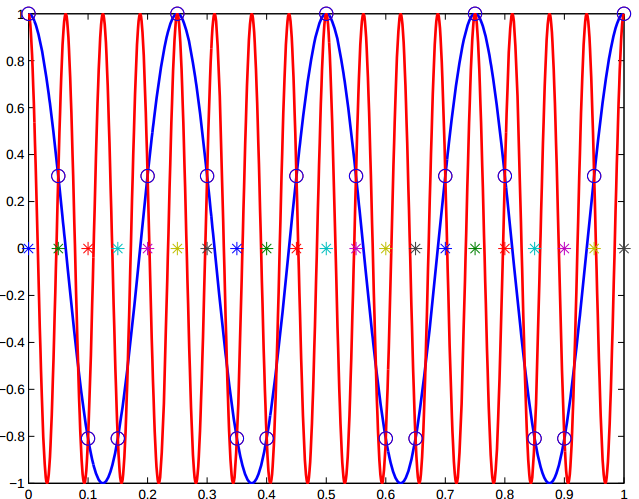
\includegraphics[width=\textwidth/2]{img/frecmalla.png}
	\caption{En la figura se pueden observar que para dos frecuencias distintas, en los puntos de la malla ambas tienen el mismo valor, por tanto son indistinguibles para el ordenador.}
	\label{fig:frecmalla}
\end{figure}

\color{red}{DE AQUI HACIA ALANTE HAY QUE COMPLETAR} 
 \begin{example}
 	$$\sum_{m=-\infty}^\infty A_M\lambda(m\pi)e^{im\pi x}$$
	Vamos a tomar una malla $J=20$, es decir, tenemos $21$ puntos en $[0,1]$
	Las frecuencias que tenemos son
	$m = -(J-1), -(J-2), \hdots, J = -19, -18, \hdots, 0, 1, \hdots, 20$.
	$m = 8\to A_8$
	
	$(A_8\lambda(8\pi)+A_{-32}\lambda(-32\pi)+A_{48}\lambda(48\pi))
	e^{i8\pi x}$
	
	En la figura se puede observar
	En azul $cos(8\pi x)$
	En rojo $cos(-32\pi x)$
	
	En todos los puntos de la malla, las funciones coinciden.
 \end{example}
 
 En el método explícito tenemos la restricción $\nu=\frac{\Delta t}{\Delta x ^2} \le \frac{1}{2}$
 $\Delta t \le \frac{\Delta x ^2}{2}$ En la práctica, a medida que refino la malla en $x$, tengo que aumentar muchísimo el número de pasos en tiempo para llegar al tiempo final.
 
\paragraph{Método implícito}
$$\frac{U_j^{n+1}-U_j^n}{\Delta t} = \frac{U_{j+1}^{n+1}-2U_{j}^{n+1}+U_{j-1}^{n+1}}{\Delta x^2}$$

Tenemos que el método implícito es
$$U_j^{n+1} = U_j^n + \nu \left[U_{j+1}^{n+1}-2U_{j}^{n+1}+U_{j-1}^{n+1}\right]$$

% %dibujos y matrices


Resuelvo el sistema lineal de la matriz $A$ para encontrar los valores en la primera fila.

Para cada paso en tiempo resuelvo el sistema de matriz tridiagonal. Es diagonalmente dominante:

$$||1+2\nu|\ge |-\nu|+|-\nu|$$

En matlab, para introducir $A$, introducimos sólo los 3 vectores de las diagonales. Rsolvemos el sistema por eliminación gaussiana, no es necesario pivotaje.

$Ax =f$
$x=\setminus f$

$A=(J-1)x(J-1)$
$\Delta x = \frac{1}{J}$
coste computacional $O(3*(J-1))$.

\begin{lstlisting}
	J = 20
	nu = 0.4
	
	e=ones(J-1,1);
	e=(1+2*nu)+e;
	eu=ones(J-2,1)
	eu=-nu*eu;
	ed=eu;
	eu=[0, eu];
	ed=[ed, 0];
	A=spdiags([ed e eu],-1:1,J-1,J)
\end{lstlisting}

\paragraph*{Análisis de Fourier del método implícito}

$$U_j^{n+1} = U_j^n + \nu \left[U_{j+1}^{n+1} - 2U_j^{n+1}+U_{j-1}^{n+1}\right]$$

$$U_j^n = \lambda^n e^{ik_j\Delta x}$$

$\lambda{n+1} e^{ik_j\Delta x} = \lambda^n e^{ik_j\Delta x} + \nu \left[\lambda^{n+1}e^{ik_{j+1}\Delta x} - 2\lambda^{n+1}e^{ik_j\Delta x}+\lambda^{n+1}e^{ik_{j-1}\Delta x}\right]$

Dividiendo por $\lambda^n e^{ik_j\Delta x}$

$\lambda = 1+\nu\left[\lambda e^{ik\Delta x}-2\lambda + \lambda e^{-ik\Delta x}\right]$

$\lambda =  1+\lambda \nu\left[e^{ik\Delta x} - 2 + e^{-ik\Delta x}\right]$

$\lambda = 1-4\nu\lambda sin^2(\frac{k}{2}\Delta x)$

$1 = [1+4\nu sin^2(\frac{k}{2}\Delta x)]\lambda$

$\lambda(k) = \frac{1}{1+4\nu sin^2(\frac{k}{2}\Delta x)}$


El método implícito es incondicionalmente estable
Siempre estable independientemente de los valores de $\Delta t$ y $\Delta X$.

Consistente de orden 1 $\implies$ el metodo es convergente.

\paragraph{El theta-método}

$$\frac{U_j^{n+1}-U_j^n}{\Delta t} = 
\theta \left[ \frac{U_{j+1}^n-2U_j^n+U_{j-1}^n}{(\Delta x)^2}\right] +
(1-\theta)\left[\frac{U_{j+1}^{n+1}-2U_{j}^{n+1}+U_{j-1}^{n+1}}{\Delta x^2}\right]$$

con $0\le\theta\le 1$

\begin{itemize}
\item $\theta = 0$ Método explícito $\nu \le \frac{1}{2}$
\item $\theta = 1$ Método implícito siempre de orden 1.
\end{itemize}

Otra forma de escribirlo es
$$U_j^{n+1} = U_j^n + \nu\theta\left[U_{j+1}^{n+1} - 2U_{j}^{n+1} + U_{j-1}^{n+1}\right] + \nu(1-\theta)\left[U_{j+1}^{n}-2U_{j}^{n}+U_{j-1}^{n}\right]$$

Escribiéndolo de forma matricial, tenemos
$U^{n+1} = 
\begin{bmatrix}
u_1^{n+1}\\
u_2^{n+1}\\
\vdots\\
u_{J-1}^{n+1}\\
\end{bmatrix}$

Para programar el método
%Matriz de kike

\begin{lstlisting}
	for n = 1:N
		U = B * U %Multiplicar por matriz tridiagonal O(3*(J-1)) operaciones
		U = A \ U %Resolver sistema O(3*(J-1))
	end
\end{lstlisting}
$A$ es una matriz tridiagonal y diagonalmente dominante
$$1+2\nu\theta > |-\nu\theta| + |-\nu\theta|$$

\paragraph*{Análisis de Fourier del método}

Buscamos $U_{j}^{n}$ de la forma
$U_{j}^{n} = \lambda ^n e^{ikj\Delta x}$

\begin{itemize}
	\item Sustituimos $U_{j}^{n}$ por $\lambda^n e^{ikj\Delta x}$
	\item Dividimos por $\lambda^n e^{ikj\Delta x}$
\end{itemize}

Nos quda

$\lambda = 1+ \nu\theta\lambda\left[e^{ik\Delta x}-2+e^{-ik\Delta x}\right] = \nu(1-\theta)\left[e^{ik\Delta x} - 2 + e^{-ik\Delta x}\right]$

Recordamos que
$e^{ik\Delta x}-2+e^{-ik\Delta x} = -4sin^2(\frac{k}{2}\Delta x)$ 

Nos queda

$\lambda = 1-4\nu\theta\lambda sin^2(\frac{k}{2}\Delta x)-4\nu(1-\theta)sin^2(\frac{k}{2}\Delta x)$

$\lambda\left[1+4\theta\nu sin^2(\frac{k}{2}\Delta x) \right] = 1 - 4\nu(1-\theta)sin^2(\frac{k}{2}\Delta x)$

$\lambda = \frac{1-4\nu(1-\theta)sin^2(\frac{k}{2}\Delta x)}{1+4\nu\theta sin^2(\frac{k}{2}\Delta x)}$

$\nu = \frac{\Delta t}{\Delta x ^ 2} \ge 0$

Cuando $|\lambda|\le 1$ ($\lambda \le 1$ siempre) pero puede ocurrirque $\lambda < -1$ y tendríamos inestabilidad.

Esto ocurre si $1-4\nu(1-\theta)sin^2(\frac{k}{2}\Delta x) < -1-4\nu\theta sin^2(\frac{k}{2}\Delta x)$

$-4\nu\theta +4\nu(1-\theta)$
$4\nu\left[1 -2\theta\right]$
$2 < 4\nu(1-2\theta)sin^2(\frac{k}{2}\Delta x)$


El caso más desfavorable es $sin^2(\frac{k}{2}\Delta x) = 1$, lo que implica $k=J\pi$

Es decir, tenemos inestabilidad $\iff 1 < 2\nu(1-2\theta)$

O lo que es lo mismo, tenemos estabilidad $\iff$ $\nu\le \frac{1}{2}(1-2\theta)^{-1}$.

En conclusión
\begin{itemize}
	\item $0\le\theta\le\frac{1}{2}$
	tenemos estabilidad $\iff$ $\nu\le\frac{1}{2}(1-2\theta)^{-1}$
	\item $\frac{1}{2}\le \theta \le 1$ 
	tenemos estabilidad siempre.
\end{itemize}

\paragraph*{Error de truncación del método}
Vamos a hacer el desarrollo de Taylor en el punto $(x_j, t_{n+\frac{1}{2}})$.

$T_j^n = \frac{u_{j}^{n+1} - u_{j}^{n}}{\Delta t} - \theta\left[\frac{u_{j+1}^{n+1}-2u_{j}^{n+1}+u_{j-1}^{n+1}}{\Delta x ^2}\right] - (1-\theta)\left[\frac{u_{j+1}^{n}-2u_{j}^{n}+u_{j-1}^{n}}{\Delta t}\right]$

1) $u_{j}^{n+1} = \left[u + \frac{1}{2}\Delta tu_t + \frac{1}{2}(\frac{1}{2}\Delta t)^2u_{tt} + \frac{1}{6}(\frac{1}{2}\Delta t)^3u_{tttt} + \hdots \right]_j^{n+\frac{1}{2}}$

$u_{j}^{n} = \left[u - \frac{1}{2}\Delta tu_t + \frac{1}{2}(\frac{1}{2}\Delta t)^2u_{tt} - \frac{1}{6}(\frac{1}{2}\Delta t)^3u_{tttt} + \hdots \right]_j^{n+\frac{1}{2}}$


$\frac{u_j^{n+1}-u_j^n}{\Delta t} = \left[u_t+\frac{1}{24}(\Delta t)^2u_{tttt}+\hdots \right]_j^{n+\frac{1}{2}}$

2) $u_{j+1}^{n+1} -2u_{j}^{n+1} + u_{j-1}^{n+1} = \left[\Delta x ^2 u_{xx} + \frac{1}{12}\Delta x ^4 u_{xxxx} + \frac{2}{6!}\Delta x ^6 u_{xxxxxx}+\hdots \right]_j^{n+1}$

$u_{j+1}^{n} -2u_{j}^{n} + u_{j-1}^{n} = \left[\Delta x ^2 u_{xx} + \frac{1}{12}\Delta x ^4 u_{xxxx} + \frac{2}{6!}\Delta x ^6 u_{xxxxxx}+\hdots \right]_j^{n}$

Desarrollos en $(x_j, t_{n+\frac{1}{2}})$.

$u_{j+1}^{n+1} -2u_{j}^{n+1} + u_{j-1}^{n+1} = \left[\Delta x ^2 u_{xx} + \frac{1}{12}\Delta x ^4 u_{xxxx} + \frac{2}{6!}\Delta x^6 u_{xxxxxx}+\hdots \right]_j^{n+\frac{1}{2}}
+ (\frac{1}{2}\Delta t) \left[\Delta x ^2 u_{xxt} + \frac{1}{12}\Delta x ^4 u_{xxxxt} +\hdots \right]_j^{n+\frac{1}{2}}
+ \frac{1}{2}(\frac{1}{2}\Delta t)^2 \left[\Delta x ^2 u_{xxtt} + \hdots \right]_j^{n+\frac{1}{2}}$

$u_{j+1}^{n} -2u_{j}^{n} + u_{j-1}^{n} = \left[\Delta x ^2 u_{xx} + \frac{1}{12}\Delta x ^4 u_{xxxx} + \frac{2}{6!}\Delta x^6 u_{xxxxxx}+\hdots \right]_j^{n+\frac{1}{2}}
- (\frac{1}{2}\Delta t) \left[\Delta x ^2 u_{xxt} + \frac{1}{12}\Delta x ^4 u_{xxxxt} +\hdots \right]_j^{n+\frac{1}{2}}
+ \frac{1}{2}(\frac{1}{2}\Delta t)^2 \left[\Delta x ^2 u_{xxtt} + \hdots \right]_j^{n+\frac{1}{2}}$

Vamos a ver lo que vale

$\theta\left[\frac{u_{j+1}^{n+1}-2u_{j}^{n+1}+u_{j-1}^{n+1}}{\Delta x ^2}\right] + (1 - \theta) \left[\frac{u_{j+1}^{n}-2u_{j}^{n}+u_{j-1}^{n}}{\Delta x ^2}\right]
= \left[u_xx + \frac{1}{12}\Delta x^2 u_{xxxx} + \frac{2}{6!}\Delta x ^4 u_{xxxxxx}  + \hdots\right]_j^{n+\frac{1}{2}} 
+(\theta - \frac{1}{2})\Delta t \left[u_xxt + \frac{1}{12}\Delta x ^2 u_{xxxx}\right]_j^{n+\frac{1}{2}}
+\frac{1}{8}\Delta t ^2\left[u_{xxtt}\right]_j^{n+\frac{1}{2}}
$

Reordenamos los términos de error

$$T_j^n = \left[(\frac{1}{2}-\sigma)\Delta t u_{xxt}- \frac{1}{12}(\Delta x)^2 u_{xxxx}\right]
+ \left[\frac{1}{24}\Delta t^2 u_{ttt}-\frac{1}{8}\Delta t ^2 u_{xxtt}\right]
+ \left[\frac{1}{12}(\frac{1}{2}-\sigma)\Delta t \Delta x^2 u_{xxxxt}\right]
- \frac{2}{6!}\Delta x ^4 u_{xxxxxx}$$

El caso general es $T_j^n = O(\Delta t)$ consistencia de orden 1.

\paragraph{Dos casos particulares}
\subparagraph{Grank Nicolson}
Es tomar $\theta = \frac{1}{2}$

Entonces
$T_j^n = -\frac{1}{12}\Delta x^2 u_{xxxx} + \frac{1}{24}\Delta t^2u_{ttt}-\frac{1}{8}\Delta t ^2u_{xxtt} - \frac{2}{6!}\Delta x ^4 u_{xxxxxx} + \hdots$

$u_t = u_xx$
$u_ttt = U_xxtt$

$T_j^n = -\frac{-1}{12}\Delta x^2 u_{xxxx} -\frac{1}{12}\Delta t^2 u_{tt} + \hdots = O(\Delta x^2 + \Delta t ^2)$

El error de consistencia en $2$ en $\Delta t$ y $Delta x$. Si $\sigma = \frac{1}{2}$ el esquema es siempre estable.
Es un método convergente de orden 2. Se puede tomar $\Delta x = \Delta t$.

\subparagraph{Se puede hacer el error de truncaçao más pequeña.}
$u_{xxt} = u_{xxxx}$

Vamos a tratar de hacer cero la suma de los dos términos.

$u_{xxt}\left[(\frac{1}{2}-\theta)\Delta t - \frac{1}{12}\Delta x^2\right] = 0$
$(\frac{1}{2}-\theta)\nu\Delta x^2 - \frac{1}{12}\Delta x^2 = 0$
$(\frac{1}{2}-\theta)\nu = \frac{1}{12}$

$T_j^n = -\frac{1}{12}\Delta t^2 u_{ttt} + \frac{1}{12}(\frac{1}{2}-\theta)\Delta t \Delta x^2u_{xxxxt}
-\frac{2}{6!}\Delta x^4 u_{xxxxxx}$

$u_{ttt} = u_{xxxxt}$
$\frac{1}{2}-\theta = \frac{1}{12}\frac{1}{\nu} = \frac{1}{12}\frac{\Delta x ^2}{\Delta t}$

%Esto se hace agrupando arriba y con uxxxxxx = uxxxxt
$T_j^n = \frac{-1}{12}\Delta t^2  u_{ttt} +\frac{1}{12}\frac{1}{20}\Delta x^4u_{xxxxt} +\hdots
= O(\Delta t^2 + O(\Delta x ^4))$

Vamos a ver si la condición $(\frac{1}{2}-\theta)\nu = \frac{1}{12}$ es compatible con la condición de estabilidad.

\begin{itemize}
	\item $0\le\theta\le\frac{1}{2} \to$ estabilidad $\iff$ $\nu\le\frac{1}{2}\frac{1}{(1-2\theta)}$
	Si tomamos $(\frac{1}{2}-\theta)\nu = \frac{1}{12} \implies (1-2\theta)\nu=\frac{1}{6}$.
	$\implies \nu=\frac{1}{6}\frac{1}{1-2\theta}\le\frac{1}{2}\frac{1}{1-2\theta}$
\end{itemize}

\paragraph{Principio del máximo y convergencia para $\nu(1-\theta) \le \frac{1}{2}$}

\begin{obs}
	La condición $\nu(1-\theta)\le\frac{1}{2}$ o $\nu\le\frac{1}{2}\frac{1}{1-\theta}$
	es más fuerte que la condición de estabilidad $\nu\le\frac{1}{2}\frac{1}{1-2\theta}$
\end{obs}

\begin{example}
	$\theta = \frac{1}{2}$ Siemore es estable pero sólo verifica el principio del máximo si $\nu\le 1$
\end{example}

\begin{theorem}
	Si se cumple la condición $\nu(1-\theta)\le\frac{1}{2}$ el $\theta$-método verifica el siguiente principio del máximo.
	$$U_{min} \le U_j^n\le U^{max}$$
	$\forall j,n$ donde 
	\begin{itemize}
		\item $U_{min} = min\{U_0^m, 0\le m\le n, U_j^0, 0 \le j \le J, U_J^m, 0 \le m \le n \}$
		\item $U_{max} = max\{U_0^m, 0\le m\le n, U_j^0, 0 \le j \le J, U_J^m, 0 \le m \le n \}$
	\end{itemize}
	
	Es decir, el máximo y el mínimo se alcanzan siempre en la condición inicial o en la frontera.
\end{theorem}
\begin{proof}
	$(1+2\theta\nu)U_j^{n+1} = \theta\nu(U_{j-1}^{n+1}+U_{j+1}^{n+1}) + (1-\theta)\nu(U_{j-1}^{n}+U_{j+1}^{n})+
	[1-2(1-\theta)\nu]U_{j}^{n}$
	
	Reducción al absurdo, razonamos con el máximo (la prueba para el mínimo sería igual).
	
	Supongo que el máximo se alcanza en $U_j^{n+1}$ para $n\ge 0$, $1\le j \le J-1$.
	
	Llamamos $U^\ast = \max\{ U_{j-1}^{n+1},U_{j+1}^{n+1},U_{j-1}^{n},U_{j+1}^{n},U_{j}^{n} \}$
	
	$(1+2\theta\nu)U_{j}^{n+1} \le \theta\nu 2U^\ast + (1-\theta)\nu 2U^\ast + [1-2(1-\theta)\nu]U^\ast$
	$2\theta\nu + 2(1-\theta) \nu + 1-2(1-\theta)\nu = 1+2\theta\nu$
	$(1+2\theta\nu)U_{j}^{n+1} \le(1+2\theta\nu)U^\ast \implies U_{j}^{n+1} \le U^\ast$
	
	$U_{j}^{n+1}$ es el máximo.
	$U^\ast = U_{j}^{n+1}$
	
	Acabo de probar que el máximo también se alcanza en $U_{j-1}^{n+1}$.
	Contradicción.
\end{proof}